\section{1174083 - Bakti Qilan Mufid}
Chapter 6 - MFCC dan Neural Network
\subsection{Teori}
\subsubsection{Jelaskan kenapa file suara harus di lakukan MFCC. delengkapi dengan ilustrasi atau gambar}
\hfill\\
Mel-Frequency Cepstral Coefficient (MFCC) itu ya cuma koefisien(bisa lebih dari satu) yang disebut Koefisien Mel Frequency. Nah, itu tu buat apa sih??. jadi gini, MFCC itu biasa digunakan dalam speech processing. lebih khususnya lagi dalam pengenalan suara atau yang lebih kerennya kita kenal dengan speech recognition. MFCC adalah metode untuk memproses sinyal suara, agar bisa kelihatan deh tu ciri-cirinya. Dilakukan proses MFCC sedemikian rupa, sehingga suatu sinyal suara bisa diekstraksi ciri2 yang membedakannya. Uniknya lagi, MFCC itu seperti pendengaran kita, karena dia memproses suara itu hampir seperti telinga kita. Tau ga sih, telinga kita itu filternya kan beda2. Kalau tinggi filternya gimana, kalau rendah gimana, nah MFCC itu seperti itu, memprosesnya secara logaritmik. Jadi Mel-Frequency Cepstral Coefficients (MFCC) dapat digunakan sebagai vektor ciri yang baik untuk merepresentasikan suara manusia dan sinyal musik. Lebih khusus lagi, MFCC telah terbukti bermanfaat untuk pengenalan suara.

\begin{figure}[H]
	\centering
	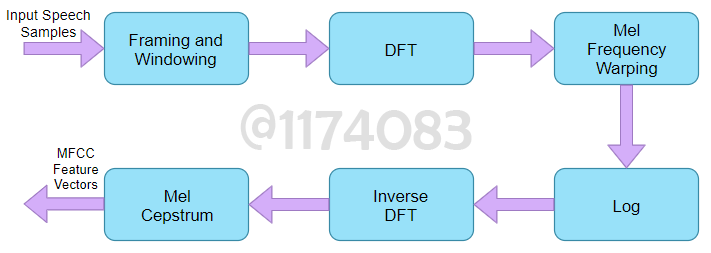
\includegraphics[width=8cm]{figures/1174083/figures6/1.png}
	\caption{gambaran penjelasan no. 1}
\end{figure}

\subsubsection{Jelaskan konsep dasar neural network.dilengkapi dengan ilustrasi atau gambar}
\hfill\\
Melalui ilustrasi di bawah bisa dilihat bahwa secara umum sebuah neural network (NN) terbagi menjadi tiga bagian, yaitu input, neuron (hidden layer) dan output. Dalam konteks deep learning, neuron memiliki istilah lain yaitu perceptron.

Input dari sebuah NN adalah variabel independen yang kita miliki. Output adalah variabel dependen yang kita cari. Misal kita ingin memprediksi harga rumah, maka variabel independennya misalnya luas tanah, luas bangunan, usia bangunan, dan lain-lain. Variabel dependennya adalah harga rumah itu sendiri. Pada contoh ini jenis output (variabel dependen) nya adalah variabel kontinu (continuous variable).

Untuk kasus yang lain, misal kita ingin mendeteksi apakah seorang calon pelanggan masuk ke kriteria target pemasaran atau tidak, maka variabel dependennya adalah berjenis binary (hanya ada 2 pilihan, ya/tidak). Jika terdiri dari lebih dari 2 kategori, maka ia masuk ke jenis kategori (categorical dependent variable). Perlu diperhatikan, jika berjenis kategori, maka outputnya juga lebih dari satu sesuai jumlah kategorinya.
\begin{figure}[H]
	\centering
	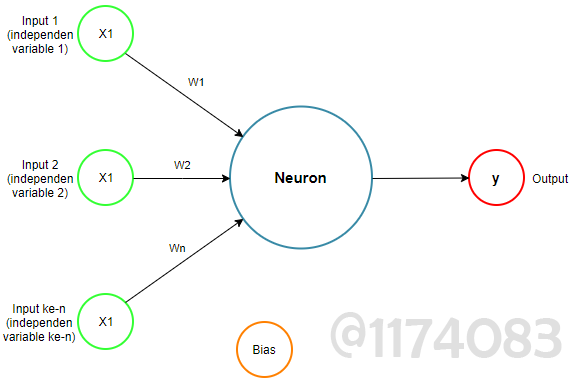
\includegraphics[width=8cm]{figures/1174083/figures6/2.png}
	\caption{gambaran penjelasan no. 2}
\end{figure}

\subsubsection{Jelaskan konsep pembobotan dalam neural network. dilengkapi dengan ilustrasi atau gambar}
\hfill\\
Setiap input memiliki nilai W yang berbeda. Bobot (weights) sangat krusial bagi neuron, karena ini merupakan bagian agar neuron bisa belajar. Nilai w (simbol untuk weights) bisa sama dan bisa juga tidak untuk setiap input yang diterima dari neuron.

Semakin besar nilai w sebuah input, maka sinyal yang berasal dari input tertentu memiliki prioritas yang semakin besar untuk bisa berkontribusi kepada neuron di depannya. Selain itu, nilai w juga menentukan apakah sinyal dari input tertentu bisa melewati neuron di depannya atau tidak.
\begin{figure}[H]
	\centering
	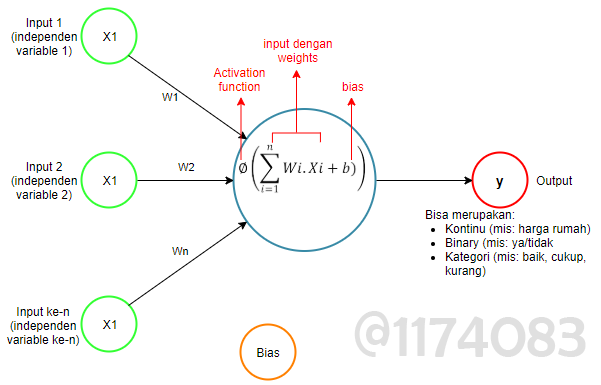
\includegraphics[width=8cm]{figures/1174083/figures6/3.png}
	\caption{gambaran penjelasan no. 3}
\end{figure}

\subsubsection{Jelaskan konsep fungsi aktifasi dalam neural network. dilengkapi dengan ilustrasi atau gambar}
\hfill\\
Fungsi aktivasi (activation function), merupakan fungsi matematis yang digunakan untuk mendapatkan output neuron dari nilai inputnya. Disebut aktivasi karena output akan bernilai jika melampaui nilai threshold-nya. Beberapa fungsi aktivasi yang sering digunakan, yaitu : 
\begin{itemize}
\item hard limiter
\item signum activation 
\item sigmoid activation.
\end{itemize} 
\begin{figure}[H]
	\centering
	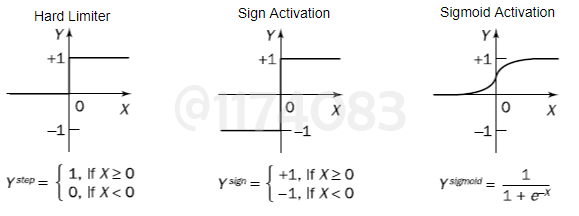
\includegraphics[width=10cm]{figures/1174083/figures6/4.png}
	\caption{gambaran penjelasan no. 4}
\end{figure}

\subsubsection{Jelaskan cara membaca hasil plot dari MFCC, dilengkapi dengan ilustrasi atau gambar}
\hfill\\
Sumbu y untuk tinggi rendah frekuensi dan sumbu x untuk lama waktu audionya. Semakin gelap warnanya, atau semakin dekat ke merah, semakin banyak daya dalam rentang frekuensi pada waktu itu.
\begin{figure}[H]
	\centering
	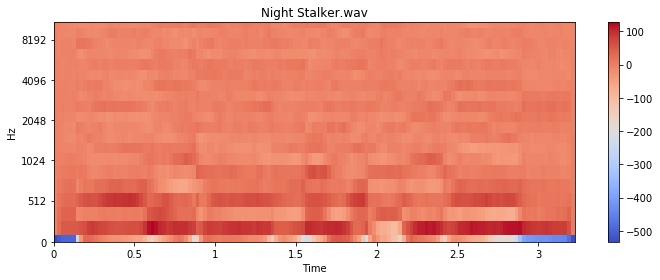
\includegraphics[width=8cm]{figures/1174083/figures6/5.png}
	\caption{gambaran penjelasan no. 5}
\end{figure}

\subsubsection{Jelaskan apa itu one-hot encoding,dilengkapi dengan ilustrasi kode dan atau gambar}
\hfill\\
one-hot encoding merupakan proses untuk mengkoversi variable categorical menjadi bentuk yang dapat diterapkan untuk Mechine Learning. 
\begin{figure}[H]
	\centering
	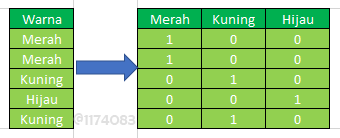
\includegraphics[width=10cm]{figures/1174083/figures6/6.png}
	\caption{gambaran penjelasan no. 6}
\end{figure}

\subsubsection{Jelaskan apa fungsi dari np.unique dan to categorical dalam kode program,dilengkapi dengan ilustrasi atau gambar}
\hfill\\
Fungsi np.unique adalah untuk mengembalikan array elemen unik dari inputan array. Contoh sebuah array [5, 2, 6, 2, 7, 5, 6, 8, 2, 9] diterapkan fungsi np.unique hasilnya menjadi [2, 5, 6, 7, 8, 9]. Fungsi to\_categorical adalah untuk mengubah nama class menjadi beberapa genre atau mengkategorikan class sesuai jenisnya.
\begin{figure}[H]
	\centering
	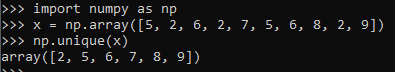
\includegraphics[width=10cm]{figures/1174083/figures6/7.png}
	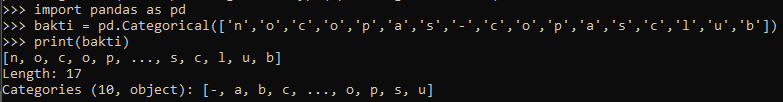
\includegraphics[width=10cm]{figures/1174083/figures6/8.png}
	\caption{gambaran penjelasan no. 7}
\end{figure}


\subsubsection{Jelaskan apa fungsi dari Sequential dalam kode program, dilengkapi dengan ilustrasi atau gambar}
\hfill\\
Fungsi dari Sequential adalah untuk memodelkan atau membuat prediksi jenis data yang sequential atau berurutan, seperti audio, teks, dan lain-lain. Contoh program untuk mengambil sepotong teks dalam bahasa Indonesia dan menerjemahkannya ke bahasa Inggris.
\begin{figure}[H]
	\centering
	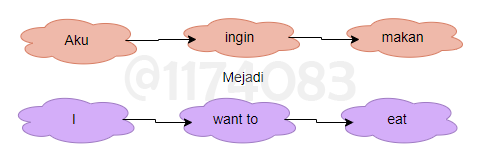
\includegraphics[width=10cm]{figures/1174083/figures6/9.png}
	\caption{gambaran penjelasan no. 9}
\end{figure}

\subsection{Praktek}
\subsubsection{Jelaskan isi dari data GTZAN Genre Collection dan data dari freesound. Buat kode program untuk meload data tersebut untuk digunakan pada MFCC. Jelaskan arti dari setiap baris kode yang dibuat(harus beda dengan teman sekelas)}
\hfill\\
Data GTZAN Genre Collection berisikan 1000 lagu dari 10 genre berbeda. Ditiap genrenya masing-masing terdapat 100 lagu yang kurang lebih durasinya 30 detik. sedangkan freesound adalah repository yang emmiliki lisensi berisikan sampel audio, contohnya suara burung, suaran drum, suara alam, dll.

Kode program untuk meload data tersebut untuk digunakan pada MFCC.
\lstinputlisting[firstline=7, lastline=17]{src/1174083/src6/1174083.py}

Import library librosa untu mengekstrak fitur dari lagu, import library glob untuk me-list file lagu ke berbagai direktori genre, import library numpy untuk melakukan operasi numerical, import library matplotlib untuk menggambar grafik MFCC,import layer dense dari library keras yang memiliki banyak neuron di dalamnya, import layer activation dari library keras untuk menggunakan activation function di tiap layer neuron, import model sequential dari library keras, import to categorical dari library keras untuk mengubah nama class menjadi beberapa genre, dan import signal dari library scipy untuk mengatasi error.

Ini spectogram dari owl-hoot(source dari freesound) yang menampilkan frekuensi rendah.
\lstinputlisting[firstline=34, lastline=34]{src/1174083/src6/1174083.py}
\begin{figure}[H]
	\centering
	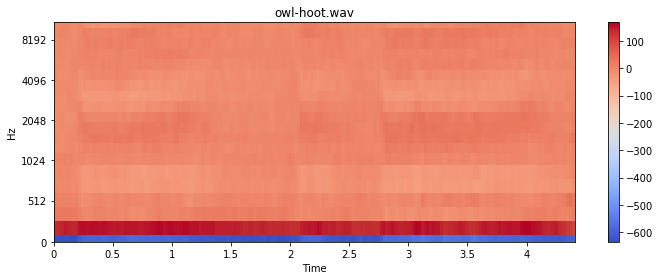
\includegraphics[width=10cm]{figures/1174083/figures6/10.png}
	\caption{spectogram owl-hoot}
\end{figure}

Ini spectogram dari the-canadian-loon(source dari freesound) yang menampilkan frekuensi rendah.
\lstinputlisting[firstline=36, lastline=36]{src/1174083/src6/1174083.py}
\begin{figure}[H]
	\centering
	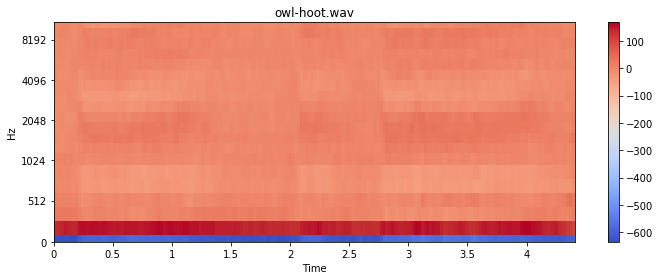
\includegraphics[width=10cm]{figures/1174083/figures6/10.png}
	\caption{spectogram the-canadian-loon}
\end{figure}

Untuk contoh spectogram dari GTZAN Genre Collection, bisa dilihat di nomor selanjutnya.

\subsubsection{Jelaskan perbaris kode program dengan kata-kata dan dilengkapi ilustrasi gambar fungsi dari display\_mfcc()}
\hfill\\
\lstinputlisting[firstline=19, lastline=28]{src/1174083/src6/1174083.py}
Membuat fungsi untuk menampilkan nilai dari MFCC dari tiap lagu. Pertama load lagunya, lalu ekstrak lagunya dengan fungsi mfcc dan tampung nilainya. Kemudian tampilkan spectogramnya dengan fungsi specshow.
\begin{itemize}
\item Nama fungsinya display mfcc() dengan parameter song untuk lagu yang nantinya diproses.
\item Fungsi load() untuk meload lagunya kemudian ditampung nilainya.
\item Fungsi mfcc() untuk mengekstrak fitur dari lagunya kemudian ditampung nilainya.
\item Fungsi figure() untuk membuat grafiknya.
\item Fungsi specshow() untuk membuat spectogramnya.
\item Fungsi colorbar() untuk memberi warna pada grafiknya.
\item Fungsi title() untuk memberi judul pada grafiknya.
\item Fungsi tight layout() untuk menyesuaikan grafiknya sesuai layout.
\item Fungsi show() untuk menampilkan grafiknya.
\end{itemize}
berikut adalah beberapa contoh penggunaan display\_mfcc(), beserta contoh data dari GTZAN Genre Collection

Ini spectogram dari lagu genre blues (source dari GTZAN Genre Collection).
\lstinputlisting[firstline=38, lastline=38]{src/1174083/src6/1174083.py}
\begin{figure}[H]
	\centering
	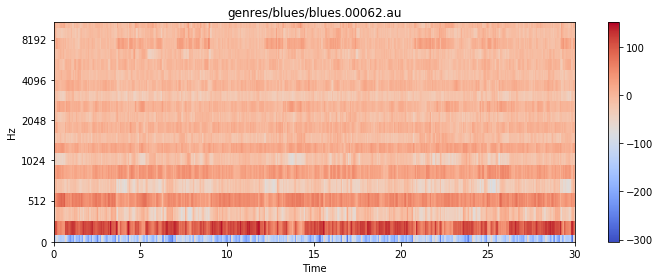
\includegraphics[width=10cm]{figures/1174083/figures6/12.png}
	\caption{spectogram dari lagu genre blues}
\end{figure}

Ini spectogram dari lagu genre classical (source dari GTZAN Genre Collection).
\lstinputlisting[firstline=40, lastline=40]{src/1174083/src6/1174083.py}
\begin{figure}[H]
	\centering
	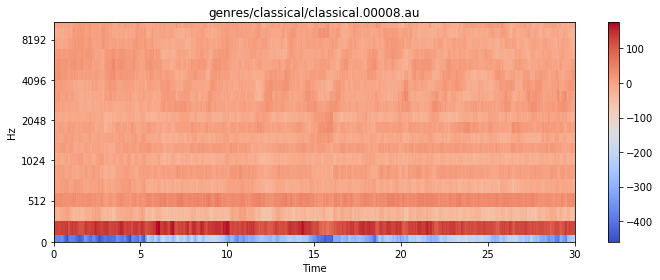
\includegraphics[width=10cm]{figures/1174083/figures6/13.png}
	\caption{spectogram dari lagu genre classical}
\end{figure}

Ini spectogram dari lagu genre country (source dari GTZAN Genre Collection).
\lstinputlisting[firstline=42, lastline=42]{src/1174083/src6/1174083.py}
\begin{figure}[H]
	\centering
	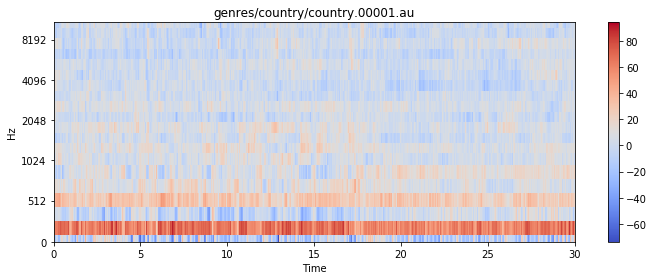
\includegraphics[width=10cm]{figures/1174083/figures6/14.png}
	\caption{spectogram dari lagu genre country}
\end{figure}

Ini spectogram dari lagu genre disco (source dari GTZAN Genre Collection).
\lstinputlisting[firstline=44, lastline=44]{src/1174083/src6/1174083.py}
\begin{figure}[H]
	\centering
	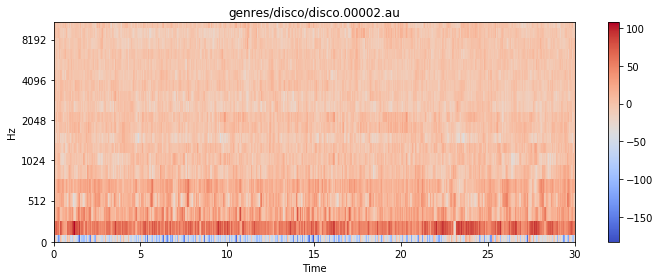
\includegraphics[width=10cm]{figures/1174083/figures6/15.png}
	\caption{spectogram dari lagu genre disco}
\end{figure}

Ini spectogram dari lagu genre hiphop (source dari GTZAN Genre Collection).
\lstinputlisting[firstline=46, lastline=46]{src/1174083/src6/1174083.py}
\begin{figure}[H]
	\centering
	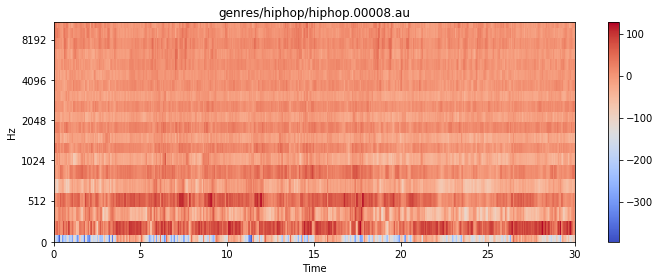
\includegraphics[width=10cm]{figures/1174083/figures6/16.png}
	\caption{spectogram dari lagu genre hiphop}
\end{figure}

Ini spectogram dari lagu genre jazz (source dari GTZAN Genre Collection).
\lstinputlisting[firstline=48, lastline=48]{src/1174083/src6/1174083.py}
\begin{figure}[H]
	\centering
	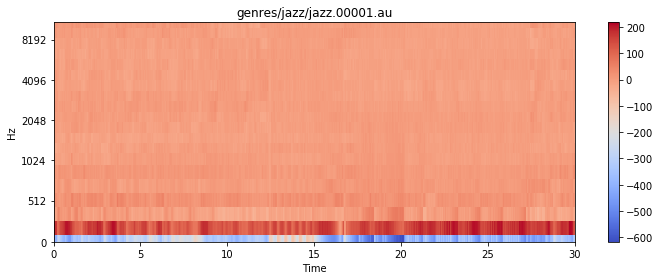
\includegraphics[width=10cm]{figures/1174083/figures6/17.png}
	\caption{spectogram dari lagu genre jazz}
\end{figure}

Ini spectogram dari lagu genre metal (source dari GTZAN Genre Collection).
\lstinputlisting[firstline=50, lastline=50]{src/1174083/src6/1174083.py}
\begin{figure}[H]
	\centering
	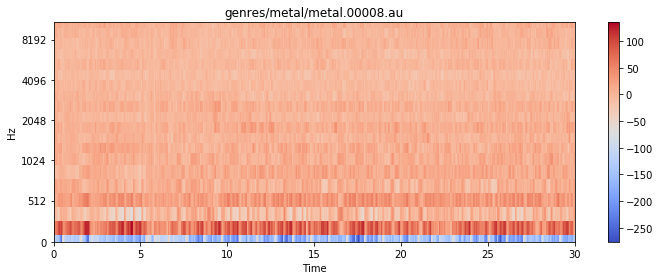
\includegraphics[width=10cm]{figures/1174083/figures6/18.png}
	\caption{spectogram dari lagu genre metal}
\end{figure}

Ini spectogram dari lagu genre pop (source dari GTZAN Genre Collection).
\lstinputlisting[firstline=52, lastline=52]{src/1174083/src6/1174083.py}
\begin{figure}[H]
	\centering
	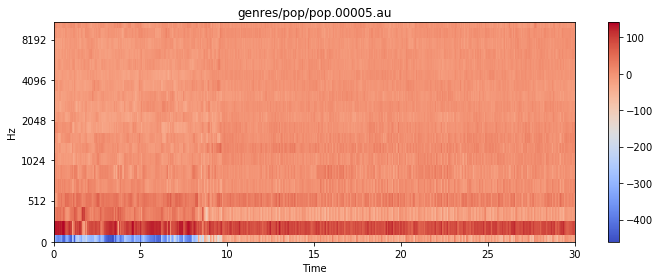
\includegraphics[width=10cm]{figures/1174083/figures6/19.png}
	\caption{spectogram dari lagu genre pop}
\end{figure}

Ini spectogram dari lagu genre reggae (source dari GTZAN Genre Collection).
\lstinputlisting[firstline=54, lastline=54]{src/1174083/src6/1174083.py}
\begin{figure}[H]
	\centering
	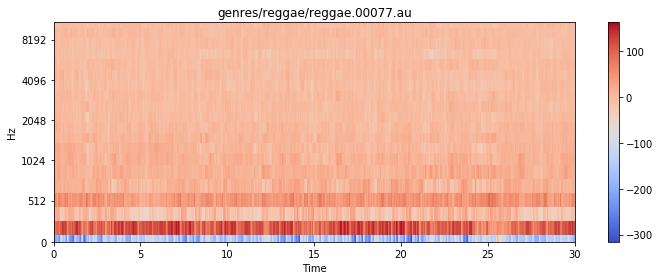
\includegraphics[width=10cm]{figures/1174083/figures6/20.png}
	\caption{spectogram dari lagu genre reggae}
\end{figure}

Ini spectogram dari lagu genre rock (source dari GTZAN Genre Collection).
\lstinputlisting[firstline=56, lastline=56]{src/1174083/src6/1174083.py}
\begin{figure}[H]
	\centering
	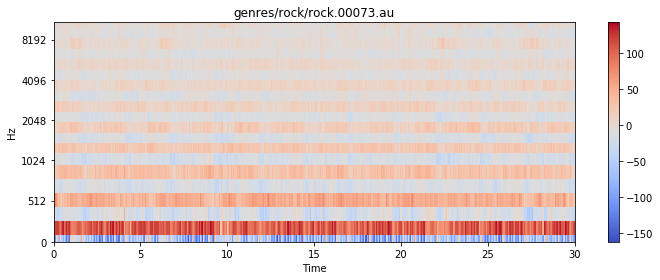
\includegraphics[width=10cm]{figures/1174083/figures6/21.png}
	\caption{spectogram dari lagu genre rock}
\end{figure}


\subsubsection{Jelaskan perbaris kode program dengan kata-kata dan dilengkapi ilustrasi gambar fungsi dari extract\_features\_song(). Jelaskan juga mengapa yang diambil 25.000 baris pertama?}
\hfill\\
Kode :
\lstinputlisting[firstline=58, lastline=66]{src/1174083/src6/1174083.py}

\begin{itemize}
	\item nama fungsinya adalah extracf\_features\_song() dengan paramete f untuk lagu yang nantinya diproses.
	\item fungsi load() untuk meload lagunya kemudian ditampung nilainya.
	\item fungsi mfcc() untuk mengekstrak fitur dari lagunya kemudian ditampung nilainya.
	\item fungsi absolute() untuk menjadikannya nilai absolut. Panggil fungsi amax untuk mencari nilai max. Kemudian hasil tadi dibagi dengan nilai mfcc sebelumnya.
	\item lalu mengembalikan hasil convert array ke dalam bentuk satu dimensi dari nilai mfcc dan diambil 25000 baris pertama.
\end{itemize}
Alasan diambil 25000 baris pertama, karena setiap lagu memiliki panjang nilai MFCC yang berbeda-beda dan yang dimasukkan ke dalam neuron harus memiliki ukuran yang sama.
\begin{figure}[H]
	\centering
	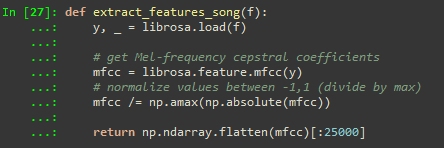
\includegraphics[width=10cm]{figures/1174083/figures6/22.png}
	\caption{Hasil dari kode program praktek nomor 3}
\end{figure}

\subsubsection{Jelaskan perbaris kode program dengan kata-kata dan dilengkapi ilustrasi gambar fungsi dari generate\_features\_and\_labels()}
\hfill\\
Kode :
\lstinputlisting[firstline=68, lastline=86]{src/1174083/src6/1174083.py}

Kode di atas dapat digunakan untuk melakukan fungsi yang sebelumnya telah kita lakukan. Kemudian di bagian genre yang disesuaikan dengan dataset nama folder. Untuk baris berikutnya akan mengulang genre folder dengan ekstensi .au. Maka itu akan memanggil fungsi ekstrak lagu. Setiap file dalam folder itu akan diekstraksi menjadi vektor dan akan ditambahkan ke fitur. Dan fungsi yang ditambahkan adalah untuk menumpuk file yang telah di-vektor-kan.
\begin{figure}[H]
	\centering
	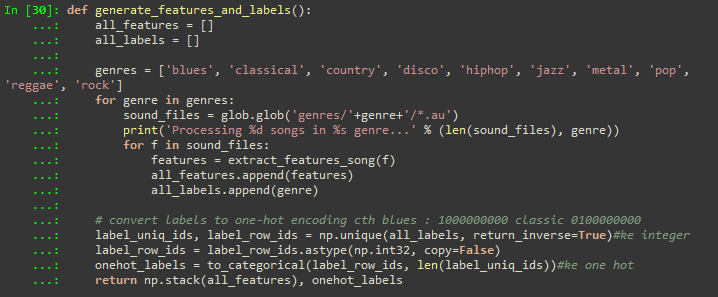
\includegraphics[width=10cm]{figures/1174083/figures6/23.png}
	\caption{Hasil dari kode program praktek nomor 4}
\end{figure}

\subsubsection{Jelaskan dengan kata dan praktek kenapa penggunaan fungsi generate\_features\_and\_labels() sangat lama ketika meload dataset genre. Tunjukkan keluarannya dari komputer sendiri dan artikan maksud setiap luaran yang didapatkan}
\hfill\\
Kode :
\lstinputlisting[firstline=88, lastline=92]{src/1174083/src6/1174083.py}

Kode diatas berfungsi untuk melakukan load variabel features dan labels. Mengapa memakan waktu yang lama ? Karena mesin akan melakukan vektorisasi terhadap semua file yang berada pada setiap foldernya, di sini terdapat 10 folder dengan masing-masing folder terdiri atas 100 buah lagu, setiap lagu tersebut akan dilakukan vektorisasi atau ekstraksi data menggunakan mfcc. Oleh karena itu, proses cukup memakan waktu.
\begin{figure}[H]
	\centering
	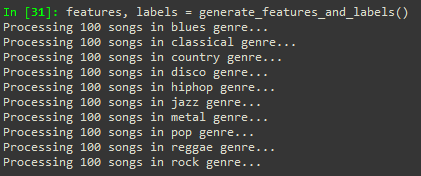
\includegraphics[width=6cm]{figures/1174083/figures6/24.png}
	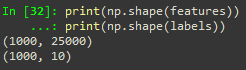
\includegraphics[width=4cm]{figures/1174083/figures6/26.png}
	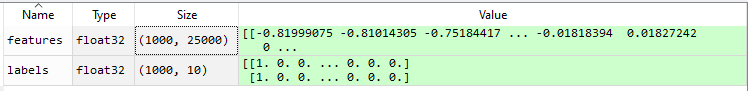
\includegraphics[width=10cm]{figures/1174083/figures6/25.png}
	\caption{Hasil dari kode program praktek nomor 5}
\end{figure}

\subsubsection{Jelaskan kenapa harus dilakukan pemisahan data training dan data set sebesar 80\%? Praktekkan dengan kode dan Tunjukkan keluarannya dari komputer sendiri dan artikan maksud setiap luaran yang didapatkan}
\hfill\\
Kode :
\lstinputlisting[firstline=94, lastline=113]{src/1174083/src6/1174083.py}

Dilakukannya pemisahan data training dan data set sebesar 80\% agar model yang dihasilkan lebih akurat dan meminimalisir kesalahan dalam pembelajaran mesin.
\begin{figure}[H]
	\centering
	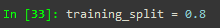
\includegraphics[width=5cm]{figures/1174083/figures6/27.png}
	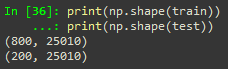
\includegraphics[width=5cm]{figures/1174083/figures6/31.png}
	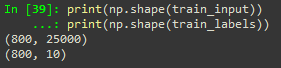
\includegraphics[width=5cm]{figures/1174083/figures6/34.png}
	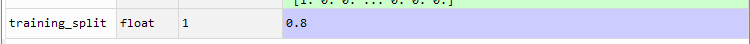
\includegraphics[width=12cm]{figures/1174083/figures6/28.png}
	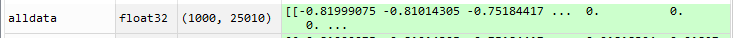
\includegraphics[width=12cm]{figures/1174083/figures6/29.png}	
	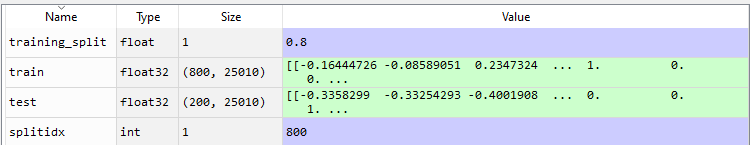
\includegraphics[width=12cm]{figures/1174083/figures6/30.png}		
	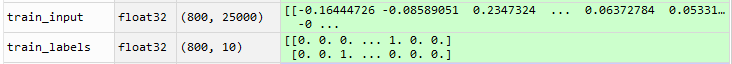
\includegraphics[width=12cm]{figures/1174083/figures6/32.png}
	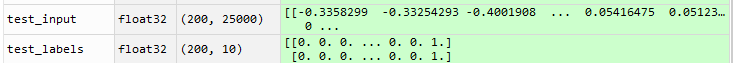
\includegraphics[width=12cm]{figures/1174083/figures6/33.png}			
	\caption{Hasil dari kode program praktek nomor 6}
\end{figure}

\subsubsection{Praktekkan dan jelaskan masing-masing parameter dari fungsi Sequential(). Tunjukkan keluaranya dari komputer sendiri dan artikan maksud setiap luaran yang didapatkan}
\hfill\\
Kode :
\lstinputlisting[firstline=115, lastline=121]{src/1174083/src6/1174083.py}

fungsi Sequential() ialah Sebuah model untuk menentukan izin pada setiap neuron, di sini adalah 100 dense yang merupakan 100 neuron pertama dari data pelatihan. Fungsi dari relay itu sendiri adalah untuk mengaktifkan neuron atau input yang memiliki nilai maksimum. Sedangkan untuk dense 10 itu adalah output dari hasil neuron yang telah berhasil diaktifkan, untuk dense 10 diaktifkan menggunakan softmax.
\begin{figure}[H]
	\centering
	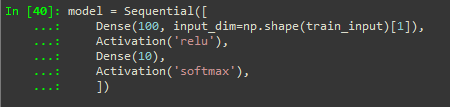
\includegraphics[width=10cm]{figures/1174083/figures6/35.png}			
	\caption{Hasil dari kode program praktek nomor 7}
\end{figure}

\subsubsection{Praktekkan dan jelaskan masing-masing parameter dari fungsi compile(). Tunjukkan keluaranya dengan fungsi summary dari komputer sendiri dan artikan maksud setiap luaran yang didapatkan}
\hfill\\
Kode :
\lstinputlisting[firstline=123, lastline=127]{src/1174083/src6/1174083.py}

Model Compile di perjelas dengan gambar dibawah, Hasil output pada kode tersebut seperti gambar menjelaskan bahwa dense pertama itu memiliki 100 neurons dengan parameter sekitar 2 juta lebih dengan aktviasi 100, jadi untuk setiap neurons memiliki masing-masing 1 aktivasi. Sama halnya seperti dense 2 memiliki jumlah neurons sebanyak 10 dengan parameter 1010 dan jumlah aktivasinya 10 untuk setiap neurons tersebut dan total parameternya sekitar 2.5 juta data yang akan dilatih pada mesin tersebut.
\begin{figure}[H]
	\centering
	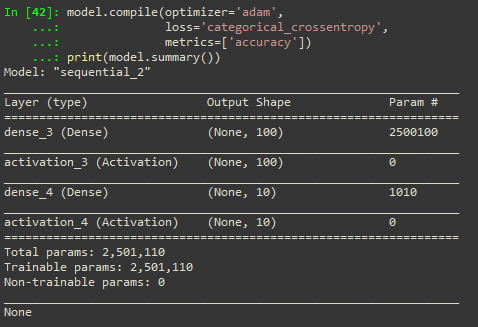
\includegraphics[width=10cm]{figures/1174083/figures6/36.png}			
	\caption{Hasil dari kode program praktek nomor 8}
\end{figure}

\subsubsection{Praktekkan dan jelaskan masing-masing parameter dari fungsi fit(). dan tunjukkan maksud setiap luaran yang didapatkan}
\hfill\\
Kode :
\lstinputlisting[firstline=129, lastline=131]{src/1174083/src6/1174083.py}

Kode tersebut berfungsi untuk melatih mesin dengan data training input dan training label. Epochs ini merupakan iterasi atau pengulangan berapa kali data tersebut akan dilakukan. Batch size ini adalah jumlah file yang akan dilakukan pelatihan pada setiap 1 kali pengulangan. Sedangkan validation split itu untuk menentukan presentase dari cross validation atau k-fold sebanyak 20\% dari masing-masing data pengulangan.
\begin{figure}[H]
	\centering
	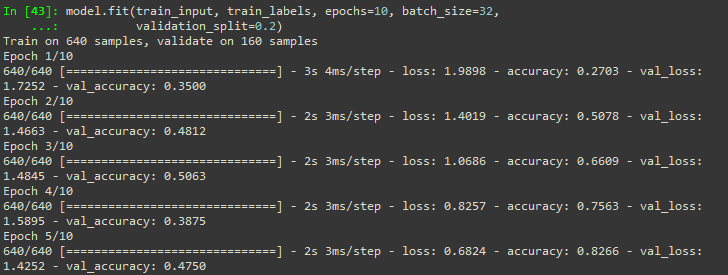
\includegraphics[width=5.5cm]{figures/1174083/figures6/37.png}		
	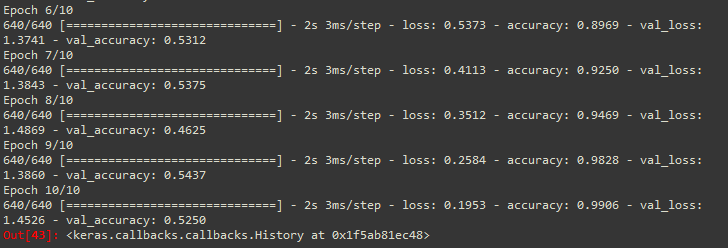
\includegraphics[width=5.5cm]{figures/1174083/figures6/38.png}	
	\caption{Hasil dari kode program praktek nomor 9}
\end{figure}

\subsubsection{Praktekkan dan jelaskan masing-masing parameter dari fungsi evaluate(). Tunjukkan keluaranya dari komputer sendiri dan artikan maksud setiap luaran yang didapatkan}
\hfill\\
Kode :
\lstinputlisting[firstline=133, lastline=137]{src/1174083/src6/1174083.py}

Fungsi evaluate atau evaluasi ini ialah untuk menguji data pengujian setiap file. Di sini ada prediksi yang hilang, artinya mesin memprediksi data, sedangkan untuk keseluruhan perjanjian sekitar 55\%.
\begin{figure}[H]
	\centering
	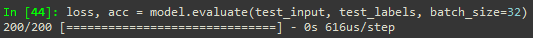
\includegraphics[width=5.5cm]{figures/1174083/figures6/39.png}			
	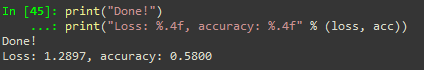
\includegraphics[width=5.5cm]{figures/1174083/figures6/40.png}	
	\caption{Hasil dari kode program praktek nomor 10}
\end{figure}

\subsubsection{Praktekkan dan jelaskan masing-masing parameter dari fungsi predict(). Tunjukkan keluaranya dari komputer sendiri dan artikan maksud setiap luaran yang didapatkan}
\hfill\\
Kode :
\lstinputlisting[firstline=139, lastline=140]{src/1174083/src6/1174083.py}

Fungsi Predict ialah untuk menghasilkan suatu nilai yang sudah di prediksi dari data training sebelumnya. Gambar dibawah ini menjelaskan file yang di jalankan tersebut termasuk ke dalam genre apa, hasilnya bisa dilihat pada gambar tersebut presentase yang paling besar yakni genre rock. Maka lagu tersebut termasuk ke dalam genre rock dengan perbandingan presentase hasil prediksi.
\begin{figure}[H]
	\centering
	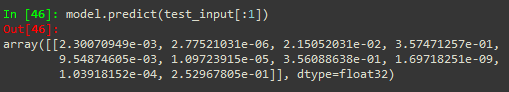
\includegraphics[width=10cm]{figures/1174083/figures6/41.png}
	\caption{Hasil dari kode program praktek nomor 11}
\end{figure}

\subsection{Penanganan Error}
\subsubsection{Terjadi error}
\hfill\\
\begin{enumerate}
\item terjadi error no module named 'librosa', seperti pada gambar berikut:
\begin{figure}[H]
	\centering
	
\includegraphics[width=8cm]{figures/1174083/figures6/error1.png}
	\caption{terjadi Error 1}
\end{figure}

\item terjadi error no module named 'keras', seperti pada gambar berikut:
\begin{figure}[H]
	\centering
	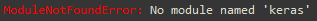
\includegraphics[width=8cm]{figures/1174083/figures6/error2.png}
	\caption{terjadi Error 2}
\end{figure}

\item terjadi error no module named 'tensorflow', seperti pada gambar berikut:
\begin{figure}[H]
	\centering
	
\includegraphics[width=8cm]{figures/1174083/figures6/error3.png}
	\caption{terjadi Error 3}
\end{figure}

\item terjadi error module 'scipy' has no attribute 'signal', seperti pada gambar berikut:
\begin{figure}[H]
	\centering
	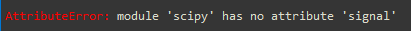
\includegraphics[width=8cm]{figures/1174083/figures6/error4.png}
	\caption{terjadi Error 4}
\end{figure}
\end{enumerate}

\subsubsection{Solusi}
\hfill\\
\begin{enumerate}
\item solusi dari error 1 ialah:
\begin{figure}[H]
	\centering
	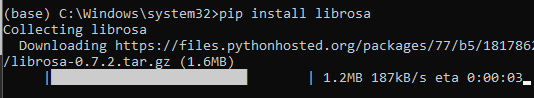
\includegraphics[width=8cm]{figures/1174083/figures6/s1.png}
	\caption{solusi error 1}
\end{figure}

\item solusi dari error 2 ialah:
\begin{figure}[H]
	\centering
	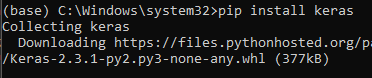
\includegraphics[width=8cm]{figures/1174083/figures6/s2.png}
	\caption{solusi error 2}
\end{figure}

\item solusi dari error 3 ialah:
\begin{figure}[H]
	\centering
	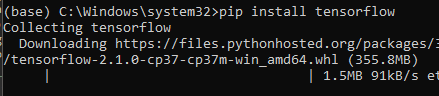
\includegraphics[width=8cm]{figures/1174083/figures6/s3.png}
	\caption{solusi error 3}
\end{figure}

\item solusi dari error 4 ialah menambahkan kode berikut:
\begin{figure}[H]
	\centering
	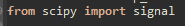
\includegraphics{figures/1174083/figures6/s4.png}
	\caption{solusi error 4}
\end{figure}
\end{enumerate}

\subsection{Bukti Tidak Plagiat}
\begin{figure}[H]
	\centering
	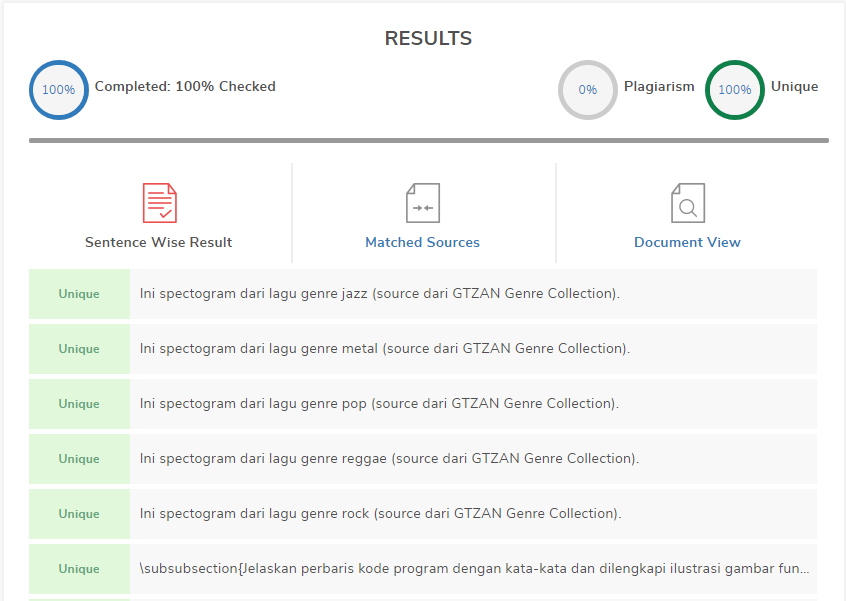
\includegraphics[width=12cm]{figures/1174083/figures6/plagiarism.png}
	\caption{Bukti tidak plagiat}
\end{figure}

\subsection{Link Youtube}
https://youtu.be/RgBkUfYZHgY